\section{Measurement alignment process, description of}
\label{sec:alignment}

\begin{figure}
\centering
\subfigure{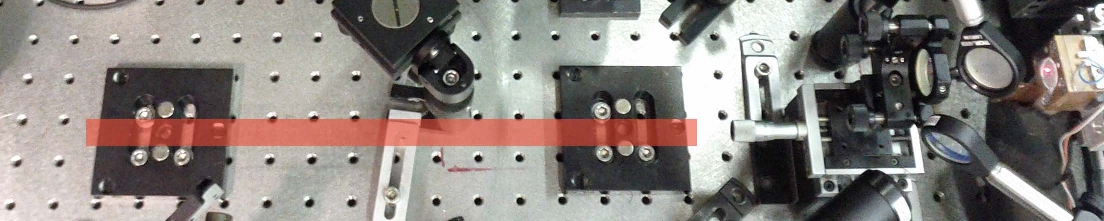
\includegraphics[width=10cm]{img/beamline_empty.jpg}}
\subfigure{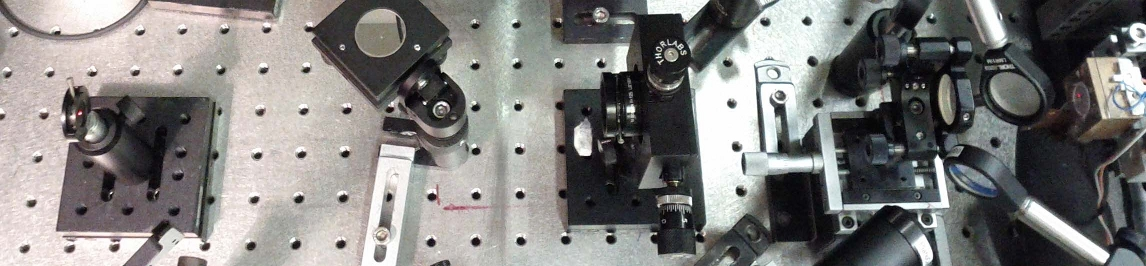
\includegraphics[width=10cm]{img/beamline_populated.jpg}}
\caption{Top: Removeable posts to define the beamline.
Bottom: HeNe beam has to be directed through the two irises.
With these two irises the position of the HeNe source is detached from the beam line.}
\label{img:beamline}
\end{figure}

The alignment process comes in two steps:
a rough base alignment
and a fine tuning.
For the first step
align the optical elements
along the emission path
to be orthogonal to it.
With the equipment
orthogonal to the beam path
we arrive
at a well-defined state,
which is easy to reproduce.

First we define the beam line.
It is defined by
two removable magnetic posts,
Fig.~\ref{img:beamline}.
These posts allow us to remove and replace a mount reproducible.
Two irises
define the beam line height.
This height
is arbitrary,
but in order to have
a reproducible setup
pick a height
and use this iris
as a reference tool.
Use the HeNe laser
for the rough alignment:
place it anywhere
on the table.
Send its beam
through the two irises;
using mirrors.
The two irises
are all we need
in order to define
the beam line.
With them
the setup is detached from the rest
of the table.

Place the sample
on the heat sink
and align it
orthogonal to the aforementioned beam line:
Remove -- or flip, Fig.~\ref{img:cavity_flipped} --
all other components along the beam line
and leave only the sample.
Adjust the orientation of the sample such that
the back-reflection is directed at the HeNe, Fig.~\ref{img:HeNe},
now it is in a well-defined configuration.
Once the sample is aligned,
place the output coupler
back in the beam path.
Repeat the same procedure.
Careful:
since the output coupler is curved
you will find two reflections.
One looks like in Fig.~\ref{img:HeNe}.
This you can align by tilting
the output coupler;
like a regular mirror.
The second reflection
is divergent.
Bring it to the center
using the xyz-translation-stage.

The last equipment
in this beam line
is the lens
after the output coupler.
It -- in combination with the output coupler --
images the sample
onto the camera
you'll use later.
Align the lens orthogonal
and choose its position
with appropriate distance
from the output couper
and camera.
Appropriate means
the picture on the camera is in focus
and there is enough room
for all the equipment.

\begin{figure}
\centering
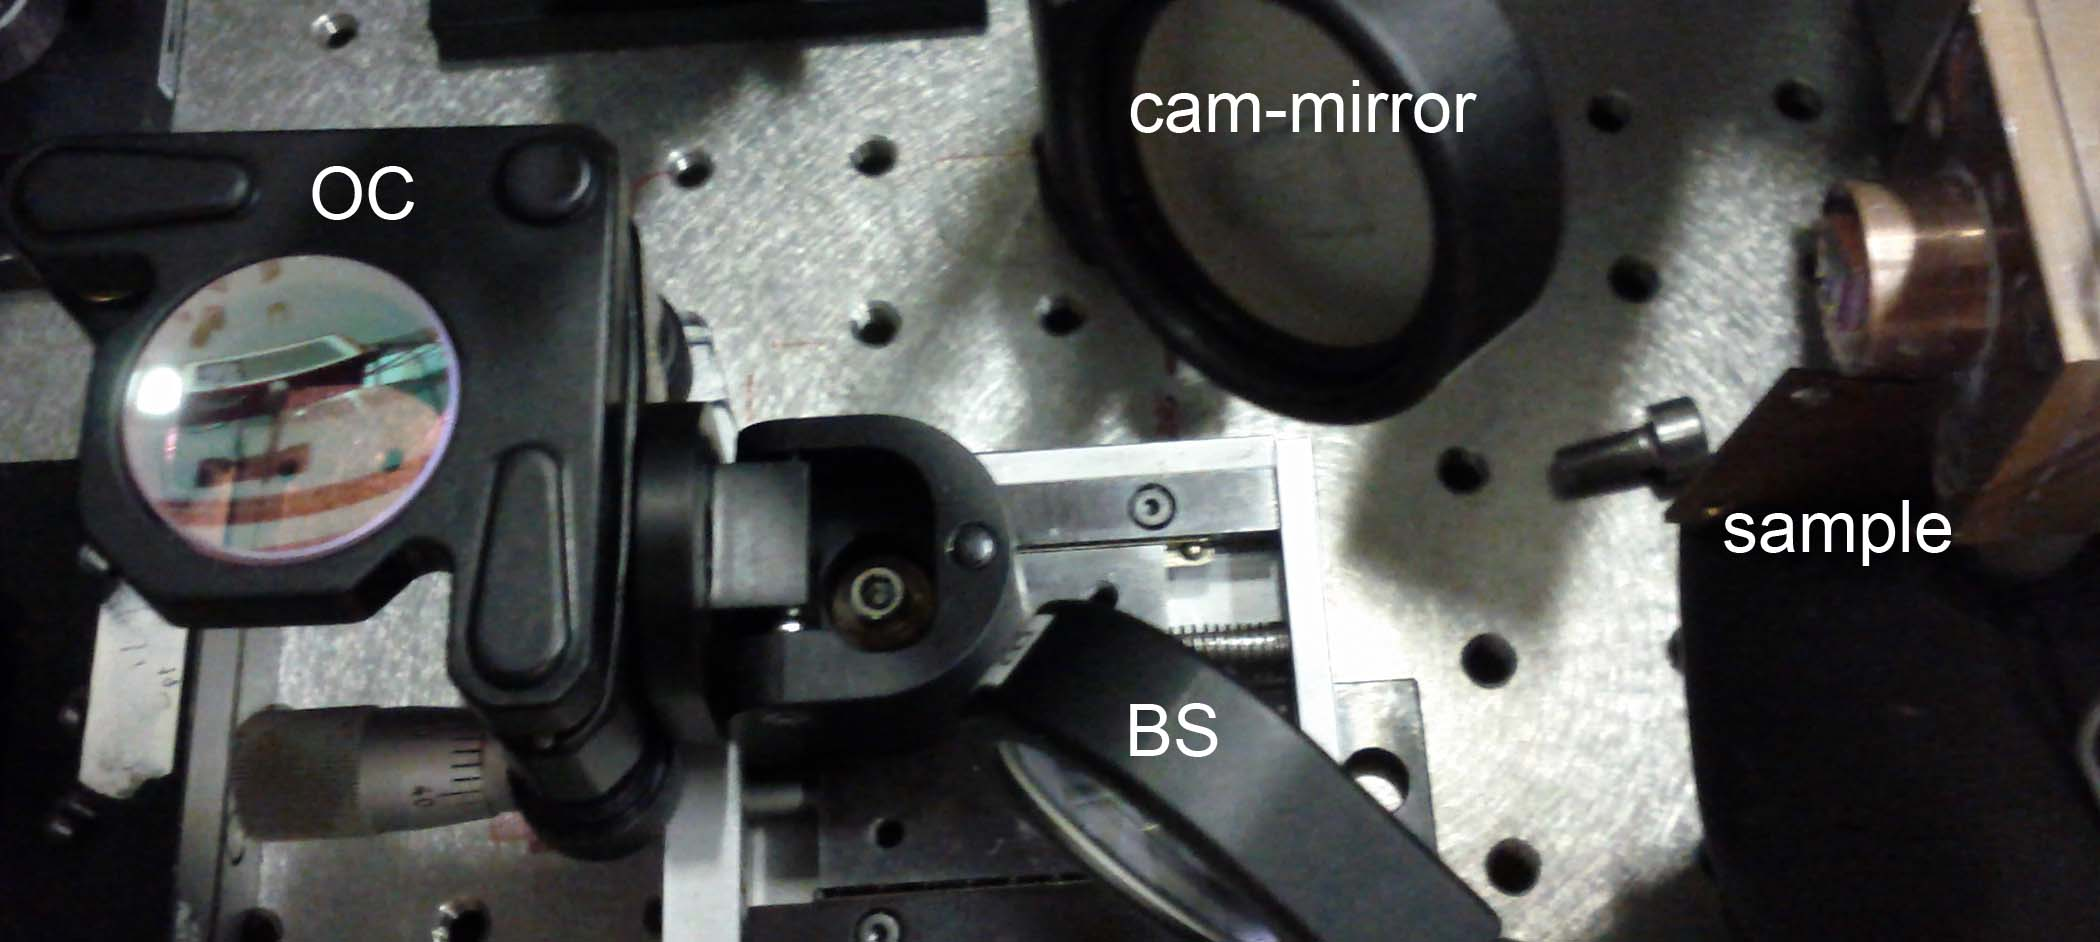
\includegraphics[width=10cm]{img/cavity_flipped.jpg}
\caption{First, we remove / flip all components along the beam line except the sample.
In this configuration we align the sample surface orthogonal to the HeNe.}
\label{img:cavity_flipped}
\end{figure}

\begin{figure}
\centering
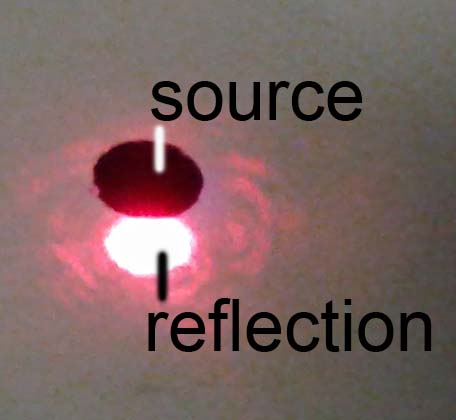
\includegraphics[width=4cm]{img/HeNe.jpg}
\caption{By arranging the reflected beam to coincide with the HeNe source position
we ensure the orthogonality of the component.
The orthogonality is an easily obtainable well-defined state,
it thus helps for reproduciblity.}
\label{img:HeNe}
\end{figure}

For the fine tuning
we need the pump light
and look at the photoluminescence
of the sample.
The camera along the emission beam line,
mentioned above,
sees the photoluminescence
resulting from the pump on the sample.
Attach a long-pass filter
to the camera
in order to see only the photoluminescence
and not the pump light.
With this camera --
initially,
thanks to the rough alignment --
we see two spots corresponding to
pump and reflection from the output coupler,
Fig.~\ref{img:spot_overlap}.
If you don't see two spots
the rough alignment
with the HeNe
was not precise enough;
repeat.
Don't forget to test whether
the sample really is
in focus of the camera.
Otherwise,
of course you won't see anything.
Bring these two spots to overlap,
using the xyz-stage of the output coupler.
Once the two spots do overlap,
and the pump is above threshold,
the sample starts lasing.
Congratulations,
the setup is aligned.

\begin{figure}
\centering
\subfigure{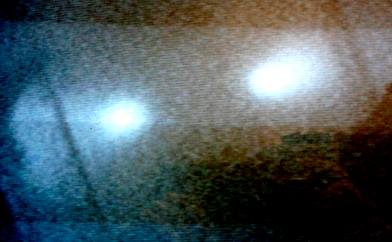
\includegraphics[width=6cm]{img/spot_overlap_two.png}}
\subfigure{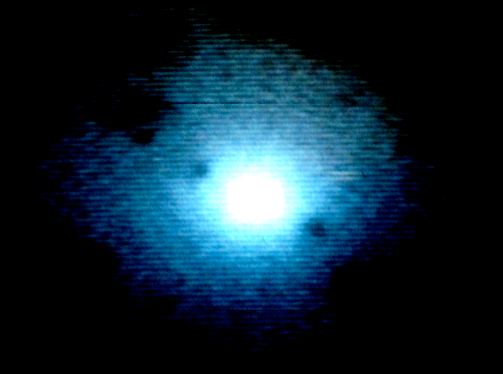
\includegraphics[width=6cm]{img/spot_overlap_one.png}}
\caption{After the pre-alignment
with the HeNe,
the two spots --
originating
from the pump
and the output coupler reflection --
are close by (left).
By optimizing the alignment
of the output coupler,
these two spots
have to be brought to overlap (right).
Given this configuration,
we have to increase the pump power,
and at threshold we obtain laser emission.
For the fine-alignment
we have to replace the camera
with a power meter
and adjust for maximum output power.}
\label{img:spot_overlap}
\end{figure}

Now you have to make sure
the beam sampler
for the pump and reflection detectors
actually send off
the sampled beam
towards the aperture
of the detectors.
If you move the pump beam sampler,
the spot moves
on the sample,
detuning the alignment
just described;
repeat.
An additional reminder
about some obvious alignment necessities:
The distance between
output coupler and sample
has to be smaller than
the radius of curvature
of the output coupler.
The distance between
pump and sample
has to match
the focal length
of the pump lens
(provided the light is collimated
after the first lens).

Figure~\ref{img:overview} shows an overview of the different components.
The pump light is directed via fiber to a lens system that images the light onto the sample.
With beam sampler BS$_p$ we extract a fraction of the pump and direct it to detector det$_p$.
This way we have a realtime reading of the pumped power.
A considerable part of the pump light is reflected off the sample.
This light diverges.
First, we thus have to collimate it.
For this we install a lens with appropriate focal length and distance from the sample.
Of this reflected beam we again sample a fraction with BS$_r$,
and direct this to detector det$_r$.
The largest fraction of the reflected beam is directed to the beam dump.
By sampling pump and reflection in this geometry
we avoid high power readings on the detectors.

\begin{figure}
\centering
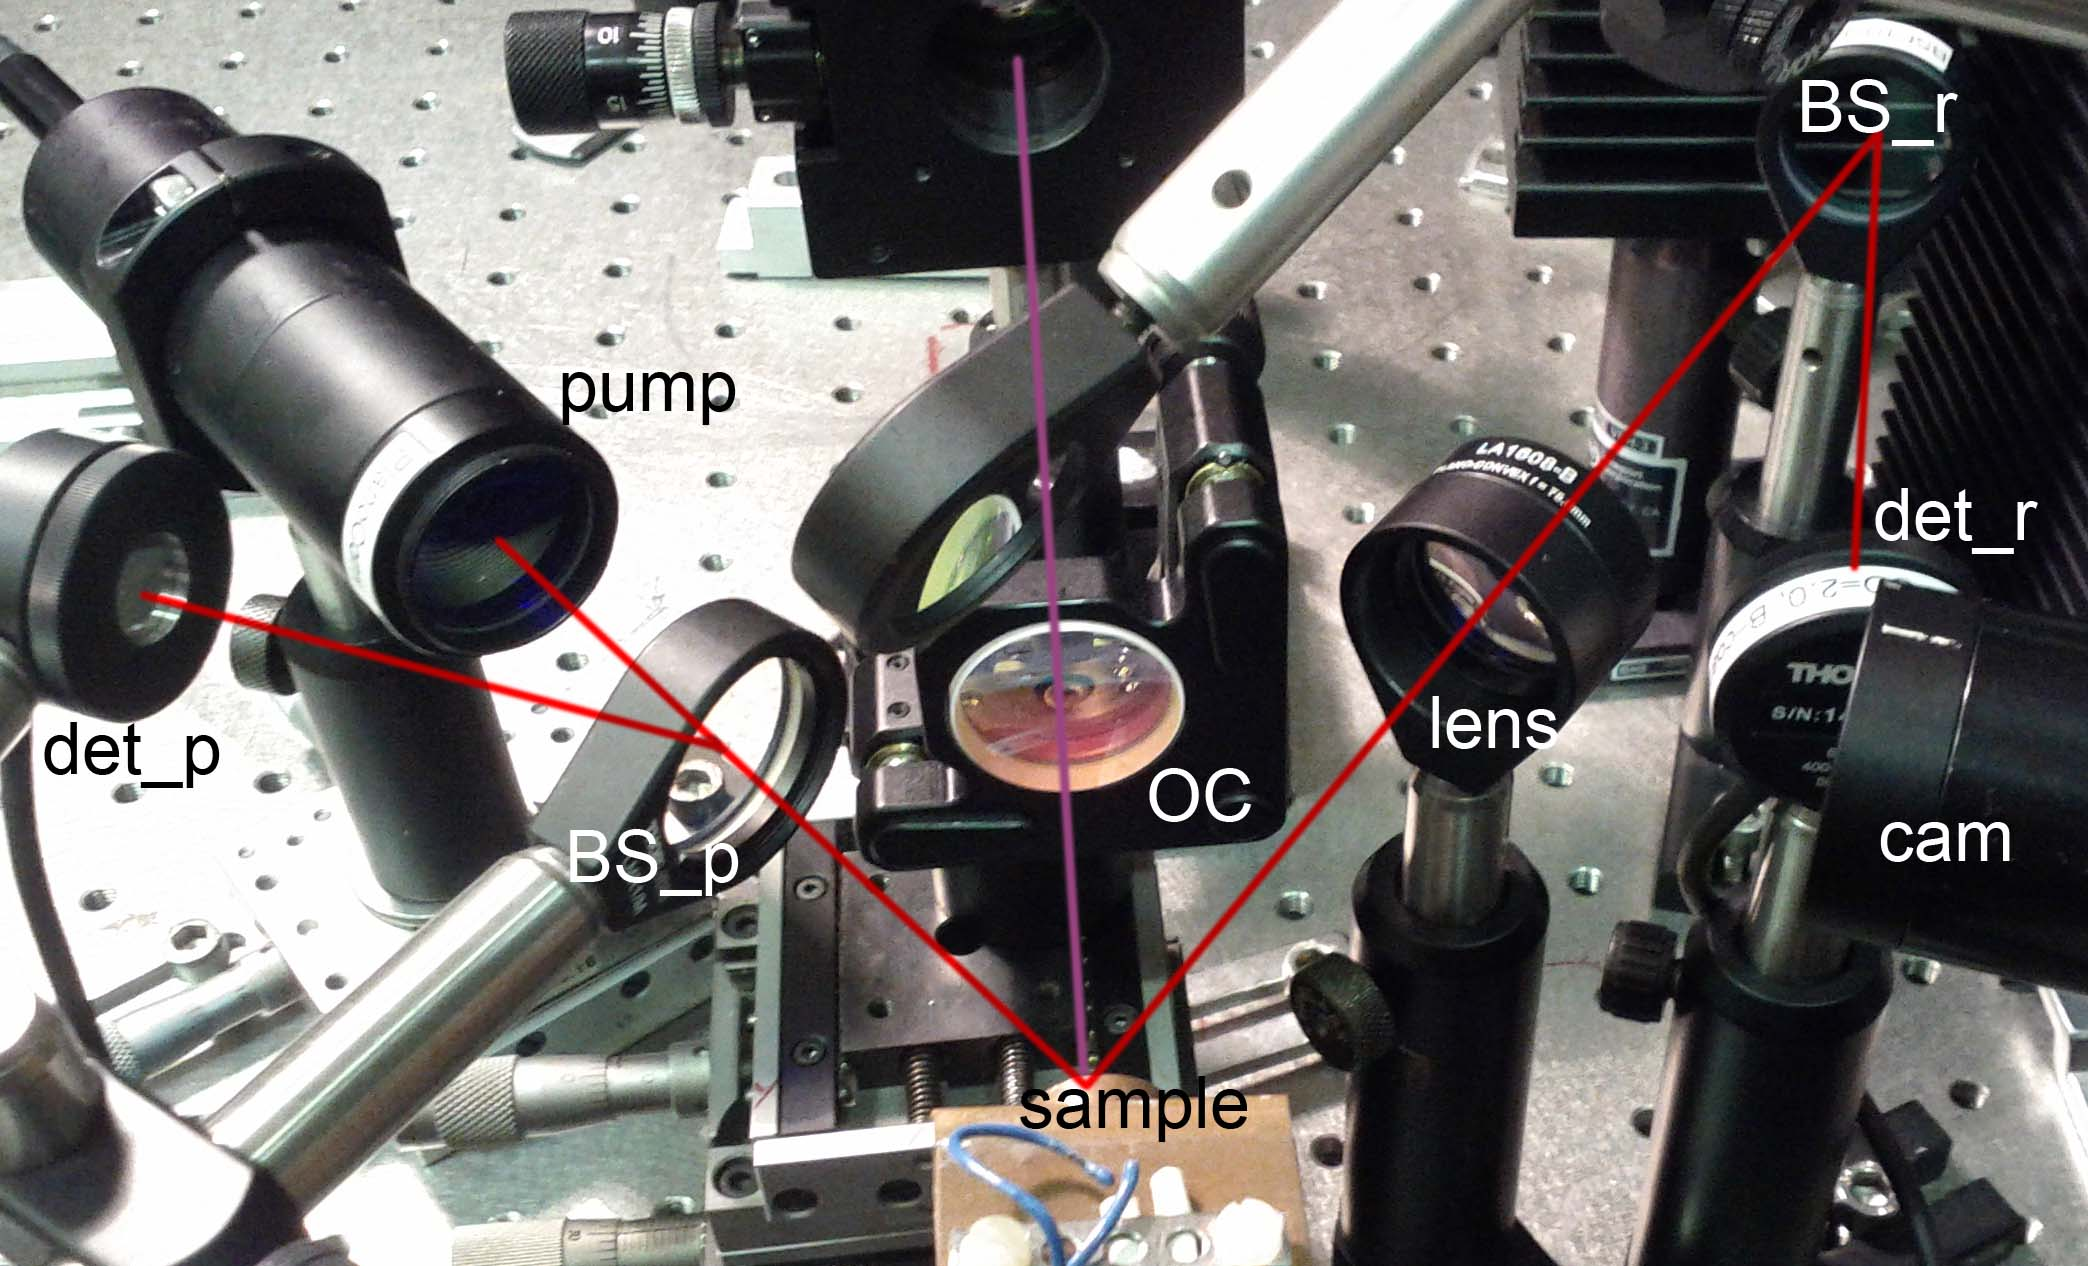
\includegraphics[width=10cm]{img/cavity_all.jpg}
\caption{Overview of the different components incorporated for the cavity.}
\label{img:overview}
\end{figure}

Before you record a measurement
you want to optimize the alignment once more:
place the power meter
in the emission path,
set the pump to a value
above threshold,
and optimize
for maximum output power.
Don't move the sample,
only adjust
the xyz-stage
of the output coupler,
and the distance between
pump and sample.
For measurements
that record the spectral information,
place also the assigned beam sampler
in the emission path.

The fiber delivering the light
to the spectrometer
is at a distance
from the sample
similar to the camera;
in the focus of the emission.
In order to have access
to both the camera
and the spectrometer
within the same setup,
several mirrors
are flippable
to use the equipment needed for the alignment step
you are at.
Coupling the emission
into the fiber
is straight forward;
but can be frustrating,
because this alignment is delicate.
You have to hit the position of the fiber core
and you have to hit
with normal incidence.
The angular component
is tricky.
We use a multimode fiber,
those allow for a larger margin of error.
Use the IR-viewer or an IR-card
to visualize the emission beam,
mount the fiber
such that is along this beam line,
and direct the beam onto the fiber.
Once you have a reading
on the spectrometer
adjust the alignment
for maximum signal.

A general note on optimizing
based on a reading on a power meter:
when you optimize the output coupler
along the cavity axis
be prepared to find more than one maximum.
Depending on the exact setting
different modes are realized.
The global maximum
performes \emph{a lot} better
than the local ones,
but it's easy to miss.
The heat sink temperature
may increase when you optimize for too long
(and thus irradiate the pump beam for a long time).
As a result the VECSEL performance
decreases and you are likely
to chase a value that isn't possible anymore,
given the new temperature.
This may lead you to find the ``maximum'' off center,
i.e. not at the maximum.
As a remedy,
take short breaks during the alignment,
or actively modify the temperature:
the maximum should be maximal also for other temperatures.
The emission power fluctuates.
This noise can pile up;
and since you scan along one parameter axis
this may also fake a wrong maximum.
In order to have a picture in mind
how that might look like,
google for ``random walk''.
You can't do anything against these error sources.
Be aware of them
and with experience in alignment
you will develop a sense for their impact.

